% This is a sample document using the University of Minnesota, Morris, Computer Science
% Senior Seminar modification of the ACM sig-alternate style. Much of this content is taken
% directly from the ACM sample document illustrating the use of the sig-alternate class. Certain
% parts that we never use have been removed to simplify the example, and a few additional
% components have been added.

% See https://github.com/UMM-CSci/Senior_seminar_templates for more info and to make
% suggestions and corrections.

\documentclass{sig-alternate}
\usepackage{color}
\usepackage[colorinlistoftodos]{todonotes}

%%%%% Uncomment the following line and comment out the previous one
%%%%% to remove all comments
%%%%% NOTE: comments still occupy a line even if invisible;
%%%%% Don't write them as a separate paragraph
%\newcommand{\mycomment}[1]{}

\begin{document}

% --- Author Metadata here ---
%%% REMEMBER TO CHANGE THE SEMESTER AND YEAR
\conferenceinfo{UMM CSci Senior Seminar Conference, December 2014}{Morris, MN}

\title{Automatic Chord Recognition from Audio}

\numberofauthors{1}

\author{
% The command \alignauthor (no curly braces needed) should
% precede each author name, affiliation/snail-mail address and
% e-mail address. Additionally, tag each line of
% affiliation/address with \affaddr, and tag the
% e-mail address with \email.
\alignauthor
Alex R. Emmons\\
	\affaddr{Division of Science and Mathematics}\\
	\affaddr{University of Minnesota, Morris}\\
	\affaddr{Morris, Minnesota, USA 56267}\\
	\email{emmon046@morris.umn.edu}
}

\maketitle
\begin{abstract}
Automatic chord recognition from audio is used in the area of music information retrieval to document and categorize music. This paper will compare the accuracy of three systems. Areas discussed include feature extraction, pre/post processing, and pattern recognition.
\end{abstract}

\keywords{Automatic chord recognition, HMM, hidden markov models, pitch class profile}

\section{Introduction}
A chord is a set of tones played simultaneously. A chord progression is a sequence of chords over time and is what forms the harmony of a piece \cite{Lee:2006}. Automatic chord recognition is the process of generating a chord progression from an audio file. Chord sequences are used by musicians as lead sheets as well as by researchers for documenting and categorizing music. Chord analysis by hand is time consuming, prone to error, and requires two or more experts. This is what makes automatic chord recognition an important area of research \cite{McVicar:2014}.

The two main steps of automatic chord recognition are feature extraction and pattern matching, with optional pre/post processing steps. Feature extraction is the process of extracting useful information from audio files and pattern matching is how chord labels are applied to that data. Preprocessing helps eliminate unwanted information from the audio files before they are analyzed.

There are many challenges that are encountered by any system that processes audio signals. There is background noise, percussive instruments, and other unwanted tones in audio recordings. It is also difficult to distinguish when a chord changes and line that up exactly with the beat.  

Chord recognition systems have been improving and becoming more usable in recent years. This paper will compare three different systems that use a variety of techniques in each step of the process. 

\todo[inline]{Need to more to these intro paragraphs, I have just provided the topic sentance for each.}   

\section{Background}

In order to explain the process of automatic chord recognition some general information about feature extraction and pattern recognition is needed. Three research cases will also be introduced.

\subsection{Feature Extraction}

The first step of generating a chord progression from audio is processing the audio signal to extract harmonic features. The pitch of a note is measured in two dimensions - height and chroma (name of the note). Height is measured in octaves and chroma tells where a note stands within the octave. A chromagram or \textit{Pitch Class Profile} (PCP) is a 12-dimensional vector representation of chroma, representing the twelve semitones in the chromatic scale. Chords are determined by the value of the notes, regardless of their height, so PCP is ideal for representing them \cite{Lee:2006}. Modern systems can have over 7 steps in converting audio to PCP including tuning correction, beat synchronization, and normalization \cite{McVicar:2014}.

Preprocessing and pre-/post-filtering are optional steps but almost all systems that I have come across use it in some way. The reason is that audio files are not perfect, they contain other tones and frequencies other than the notes being played. Musical instruments also produce what are known as overtones, tones that sound above or below the note that was played \cite{TaeMin:2014}. Preprocessing is done to the raw audio file, to remove unwanted noise and frequencies. Pre-filtering is done after the feature extraction step, in order to smooth out the PCP. Post-filtering is done after the chords have been determined by the pattern recognition step, finding the most likely sequence and eliminating unlikely chords. 

\subsection{Pattern Recognition}

Almost all chord recognition systems use PCP or some chroma-based feature extraction, what differentiates each system is the mechanism used to label chords. Generating the chord model that will be used to match the PCP against can be done in one of two ways: manually using musical knowledge or derived stochastically from real-world music. In a manual or pattern matching system, the chroma values being sounded are compared against pre-defined chord templates. the These two methods are compared by TaeMin in  \cite{TaeMin:2014}. Stochastic chord models are more sophisticated and complex. Hidden markov models used to be the method of choice but many recent systems prefer Gaussian mixture models \cite{TaeMin:2014}.

\todo[inline]{Need more here}

\subsection{Research Cases}
This paper looks at three research cases that involve automatic chord recognition. All of the cases use three common steps in the process: feature extraction, pre/post processing, and pattern recognition.

The first study \cite{Morman:2006} uses a chord recognition system that begins with a two-stage preprocessing step of Homomorphic Liftering and the use of Harmonic Product Spectrum.\todo[inline]{Define these in preprocessing section}Next is the feature extraction block where the PCP is calculated. In this case a total of 84 frequency bins are used, with the first corresponding to the lowest C on the piano. The pattern recognition step is divided into the segmentation followed by recognition of chords \cite{Morman:2006}.

The next study \cite{Lee:2006} uses a supervised HMM trained with audio-from-symbolic data. The system used here begins with feature extraction, again using PCP. At the same time, chord label data is generated from the MIDI data that was used to generate the audio. This data is used to train a 36-state HMM \cite{Lee:2006}. These 36 states represent 36 chords - major, minor, and diminished for each 12 notes. The system is trained on a group of data, and then fed a separate group of data for testing and analysis. 

The final study \cite{TaeMin:2014} compares the most common methods of each step: feature extraction, pattern recognition, and pre/post processing.   

\todo[inline]{Needs more on the second and third case}

\section{Feature Extraction}

For over a decade PCP has been the most popular way to extract harmonic features for chord recognition. Most new approaches are variations or refinements of this approach \cite{TaeMin:2014}.

\subsection{Pitch Class Profile} 

\subsection{Pre/post Processing}


\section{Pattern Recognition}

There are endless ways to assign chord labels to the PCP values, ranging from simple to very complex. We will look at two of the most common models for pattern matching chords.

\subsection{Hidden Markov Models}\label{main} 

A \textit{hidden Markov model} (HMM) is a statistical model which describes a finite set of states, in this case chords, each with a probability distribution. Transitions between these states are governed by a set of transition probabilities that describe the likelihood of transitioning from one to another \cite{TaeMin:2014}. HMMs are used in a wide variety of pattern recognition environments such as speech, handwriting, and gesture recognition, as well as in bioinformatics. 

\todo[inline]{Needs to re-write this section from draft.}

\subsection{Gaussian Mixture Models}

\textit{Gaussian mixture models} (GMMs) are used in many modern chord recognition systems. A GMM consists of a multimodal distribution of weighted Gaussian components that represent descriptions of each chord in the training data\todo[inline]{Need a better definition}. To train these models the PCP from the training data is transposed to all C-based chords (C-major and C-minor). These normalized chords are used to train the C-major and C-minor models, and then re-transposed to the remaining 11 keys~\cite{TaeMin:2014}.

\section{Research Cases}

This section describes the datasets used in each of the research cases introduced earlier.

\subsection{Effects of Proper Signal Processing}

In this experiment MIDI (Musical Instrument Digital Interface) recordings were used to create time aligned labeld audio. Two datasets were used: one of isolated chords synthesized on different instruments and one of continuous single-instrument audio synthesized as piano recordings. An overview of the system can been seen in figure~\ref{fig:fig2}. 

The isolated chord dataset consisted of 7790 chords and inversions. Three complexity levels were tested: the first involved the common triad types (major, minor, augmented, and diminished), the second included variations on the 7th (major, minor, dominant, fully diminished, and half diminished), and in the third 11 different chord types were used. The system is tested on chords that were played by the instrument it was trained on, as well as a random instrument. Four feature vectors, or models were used for comparison on each of these datasets. The first model started with preprocessing using homomorphic liftering and harmonic product spectrum. FV2 has a low sampling rate and no preprocessing, FV3 increases the sample rate and FFT length, and FV4 first preprocesses the signal and then uses the same homomorphic processing and HPS as FV1.

\todo[inline]{Need more info here.}

The continuous single-instrument audio dataset consisted of 50 hymn verses selected from the Trinity Hymnal, with 40 used for training and 10 used for testing. FV4 was used from the isolated chord experiment \cite{Morman:2006}. 

In the experiments two pattern recognition methods are compared: GMMs and Support Vector Machines (SVM). For SVM classification, the OSU SVM Classifier MATLAB Toolbox was used. 

\begin{figure}
\centering
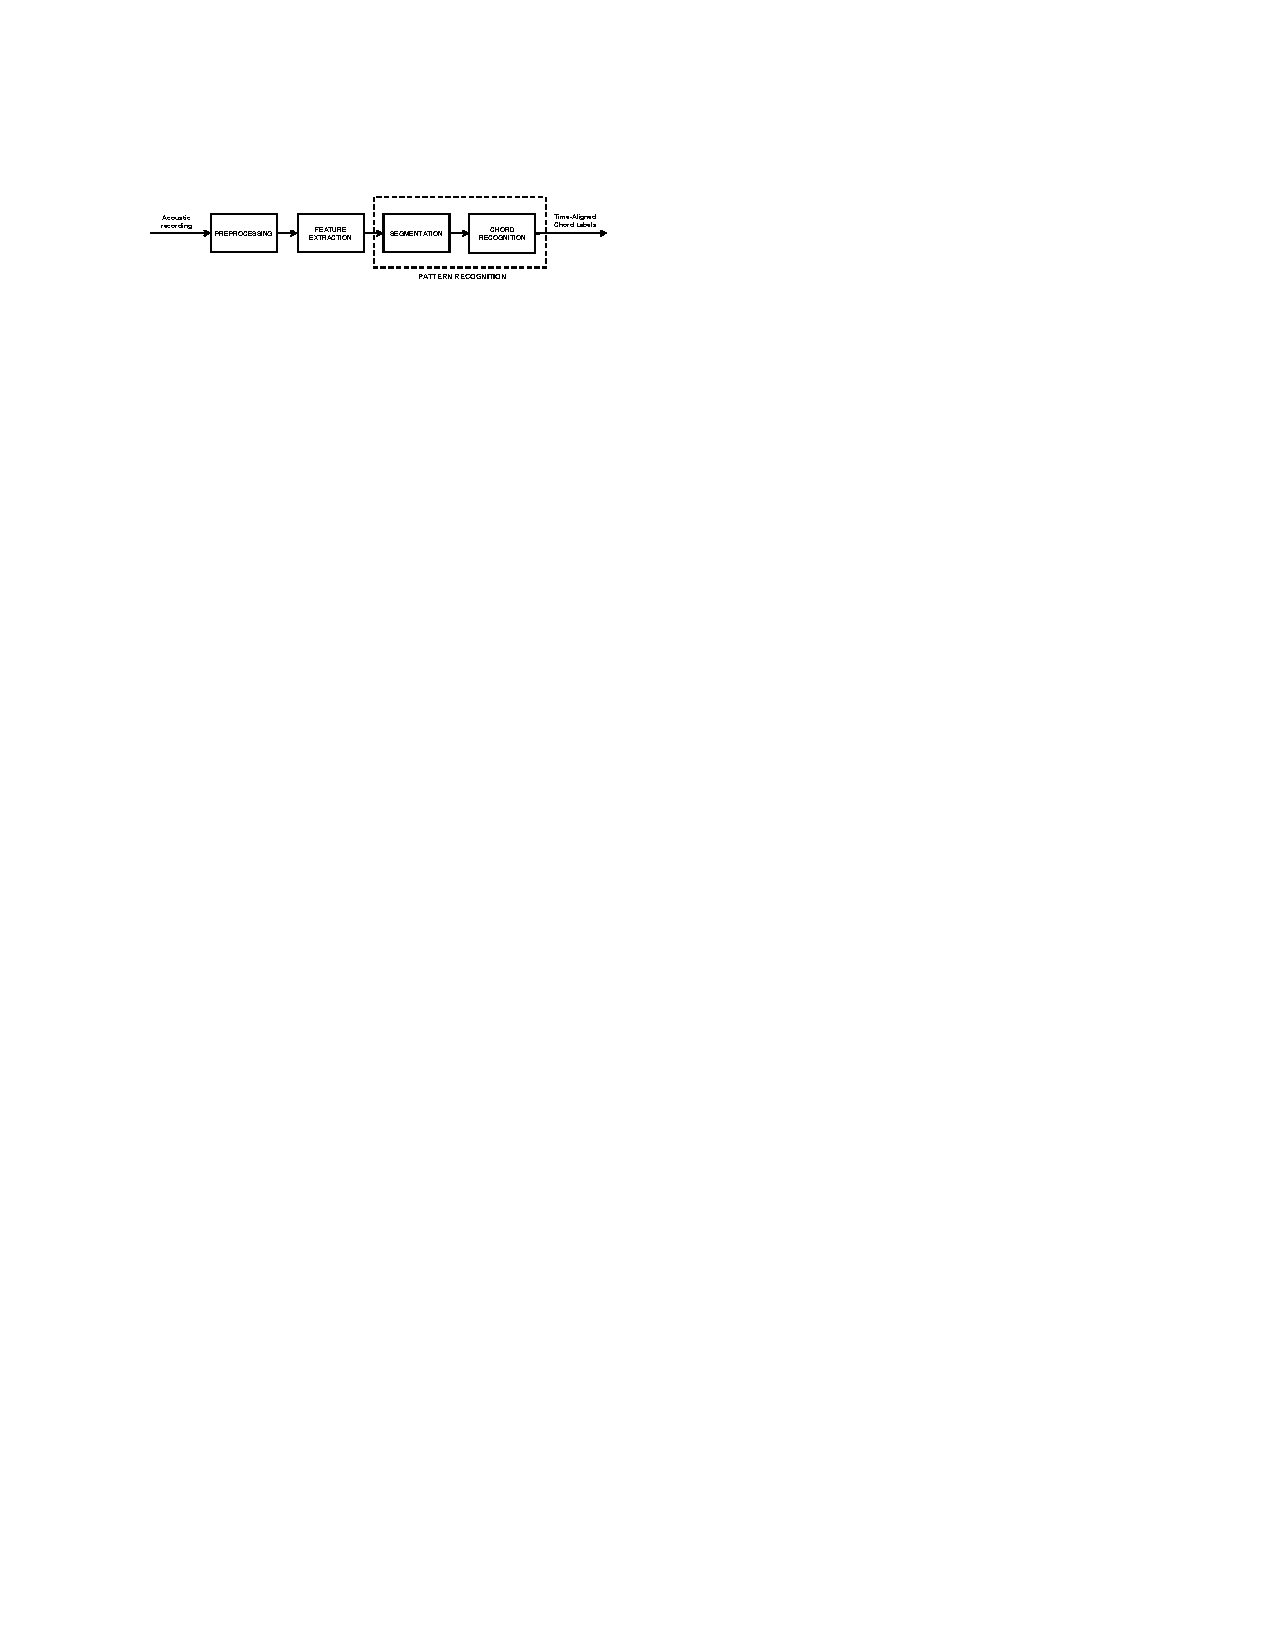
\psfig{file=fig2.pdf,width =3in}
\caption{Overview of chord recognition system used in proper signal processing study.}
\label{fig:fig2}
\end{figure}

\subsection{HMM with Audio-From-Symbolic Data}

In the HMM trained with audio-from-symbolic data \cite{Lee:2006} a 36-state HMM is used, with each state representing a single chord. Using an ergodic model, which allows every possible transition from chord to chord, the model parameters are learned and then the Viterbi algorithm is applied. The Viterbi algorithm finds the most likely path, or chord sequence, by restricting unlikely chord transitions \cite{TaeMin:2014}. Two things are needed to train this model: chord label files, and audio data. See figure~\ref{fig:fig1} for a representation of this. In this case they are both being generated from the same symbolic data. The first step is to use a chord analysis tool to generate a file with complete chord information for a piece of music. Using the same symbolic data, the audio files are generated using a sample-based synthesizer. This audio data is in perfect sync with the chord label file, and is just as good as a real recording because it contains the upper harmonics that would be generated from real instruments \cite{Lee:2006}.

\todo[inline]{Need to re-write from section draft}

The training data used for the first model in this case consisted of 81 solo piano pieces by J.S. Bach, Beethoven, and Mozart. For the second case 196 string quartet pieces by Beethoven, Haydn, and Mozart were used. The models were then test on excerpts from the Kostka and Payne's book, which includes analysis and audio recordings done by the composers. 10 excerpts - 5 piano solos and 5 string quartets were selected, with no overlap of the training data. The output was compared with the hand-marked data for frame rate accuracy \cite{Lee:2006}. 

\begin{figure}
\centering
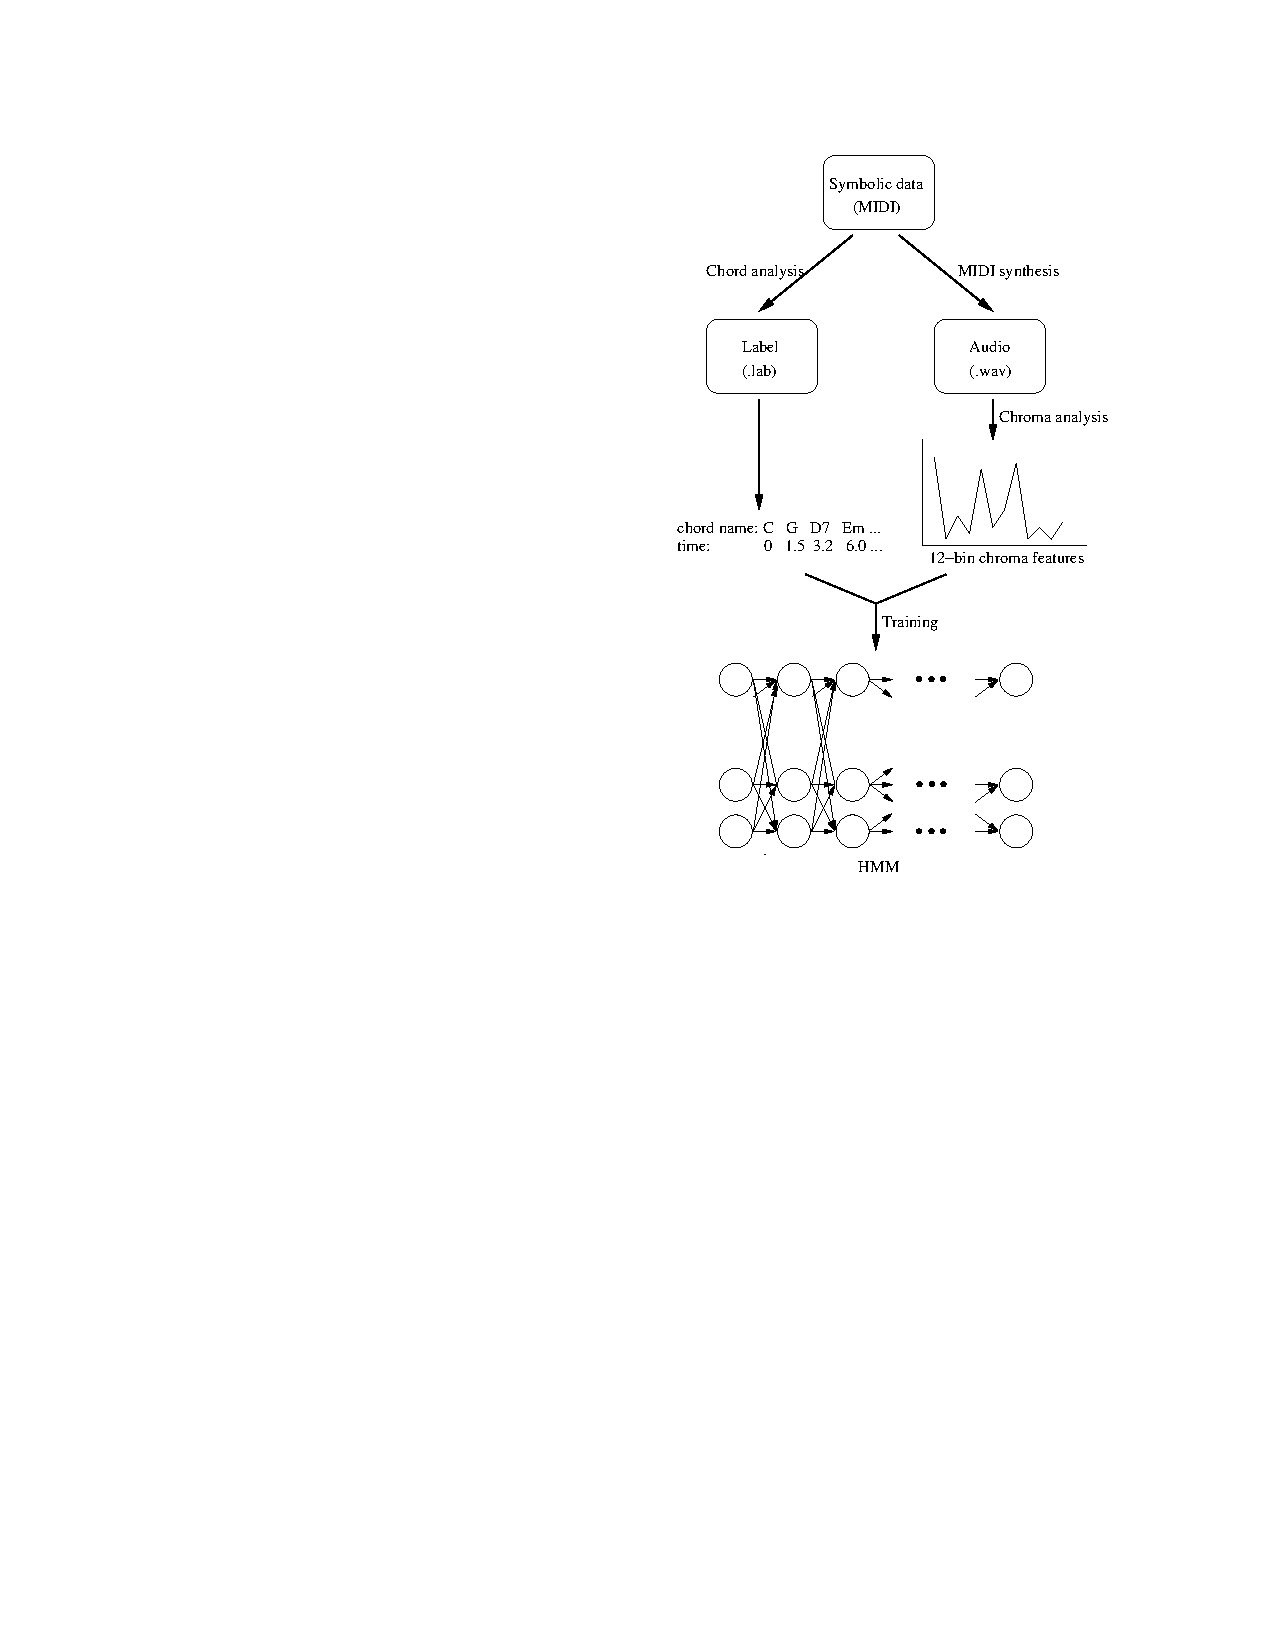
\psfig{file=fig1.pdf,width =3in}
\caption{Overview of the HMM trained with audio-from-symbolic data.}
\label{fig:fig1}
\end{figure}

\subsection{Multiple Methods}

Four experiments were conducted in this study: Feature extraction and pattern matching, effect of pre-filtering, effect of post-filtering, and combinied pre- and post-filtering. Each experiment was run on 495 chord annotated pop songs. An overview of the system can been seen in figure~\ref{fig:fig3}.

The dataset consisted of 180 Beatles songs, 20 Queen songs, 20 songs from the RWC (Real World Computing) pop dataset, and 195 songs from the US-Pop dataset. For training, 5-fold cross validation was used with each group having 99 songs selected randomly. For each fold one group is selected and the other four are used for training. Accuracy is represented by the total duration of correct chords out of the total duration of the dataset~\cite{TaeMin:2014}.

In the first experiment different combinations of feature extraction and pattern matching are compared to show whether or not model complexity affects performance of the system. They also test the effect of different types of chroma features. The second experiment looks at the pre-filtering techniques of moving filters and beat-synchronization. The effect of post-filtering experiment compares the use of different stochastic models. The final experiment uses pre- and post-filtering and again looks at moving filters and beat-synchronization.

\todo[inline]{Needs more work}

\begin{figure}
\centering
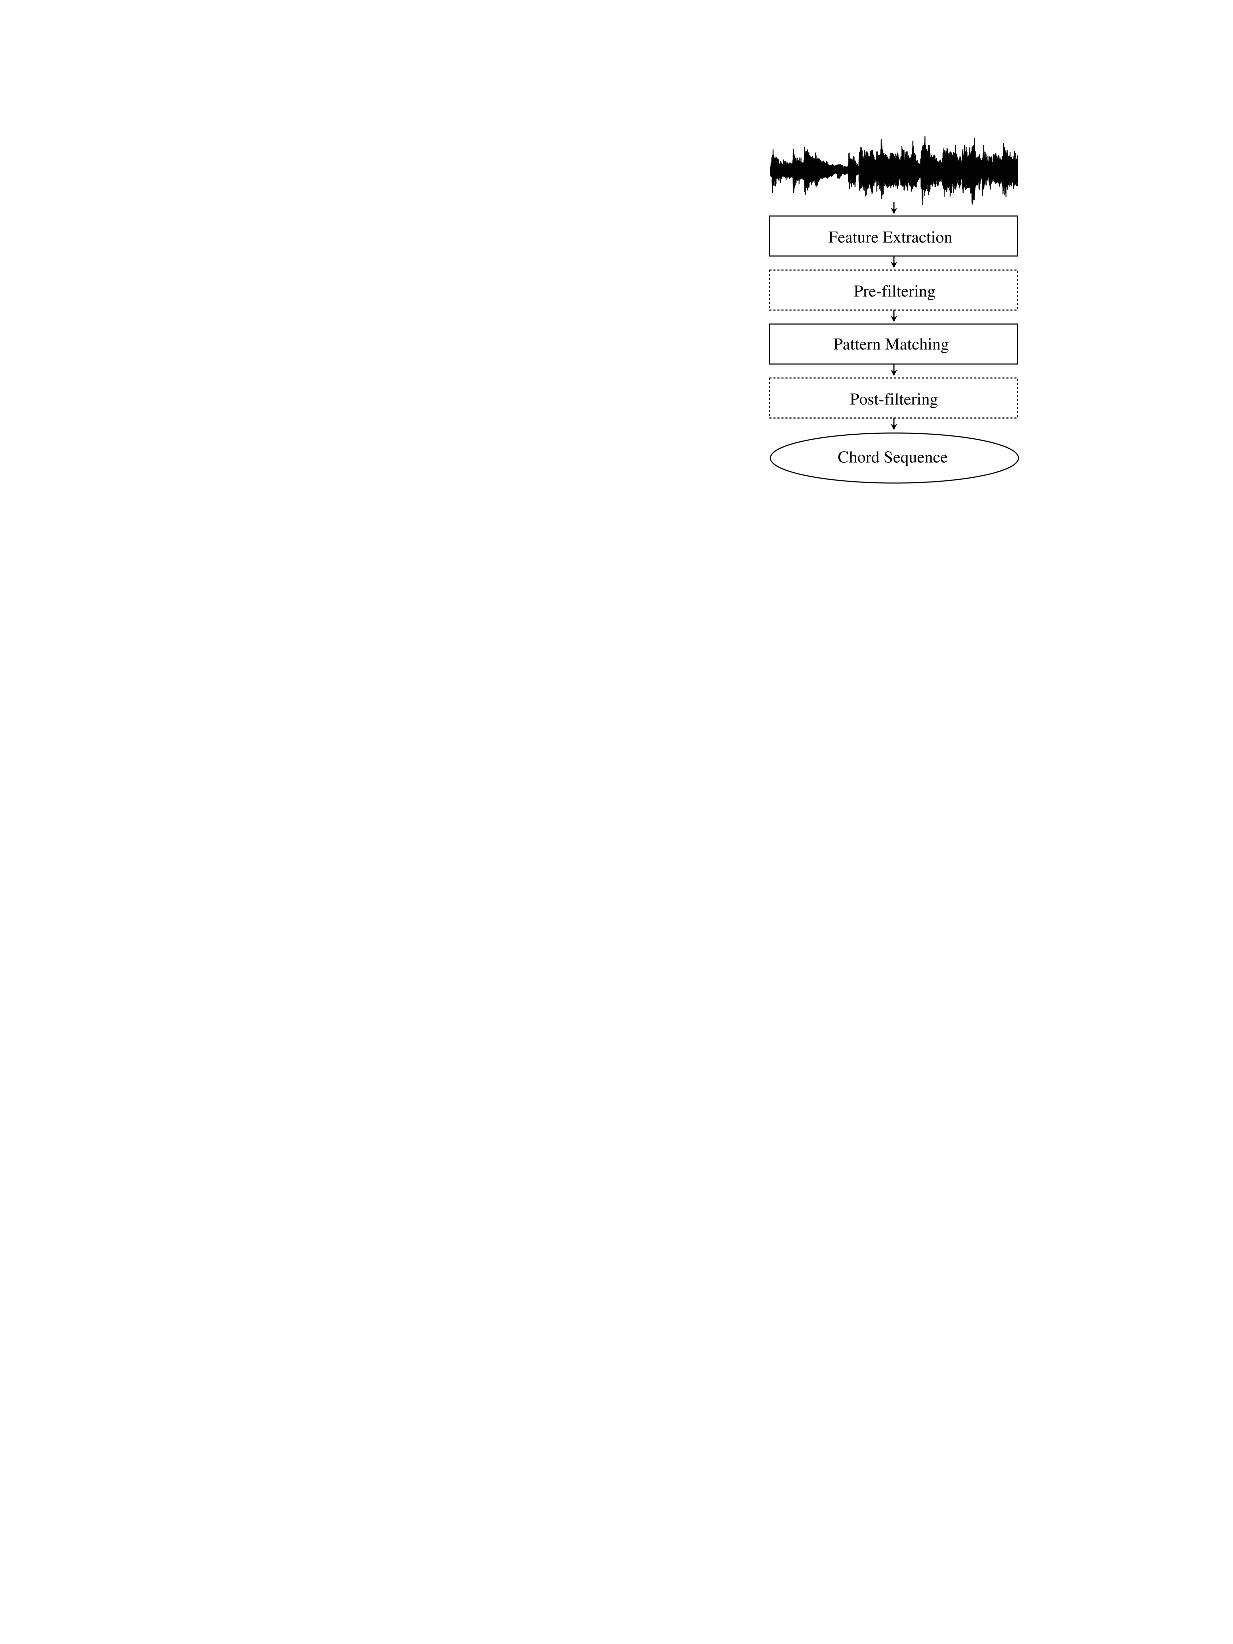
\psfig{file=fig3.pdf,width =3in}
\caption{General layout of the chord recognition system used in the multiple methods case.}
\label{fig:fig3}
\end{figure}

\section{Results}

This section describes the results of the research cases.

\subsection{Effects of Proper Signal Processing}



\subsection{HMM with Audio-From-Symbolic Data}

\subsection{Multiple Methods}

\section{Conclusions}

\section{Acknowledgements}

%\subsection{Math Equations}
%You may want to display math equations in three distinct styles:
%inline, numbered or non-numbered display.  Each of
%the three are discussed in the next sections.

%\subsubsection{Inline (In-text) Equations}
%A formula that appears in the running text is called an
%inline or in-text formula.  It is produced by the
%\textbf{math} environment, which can be
%invoked with the usual \texttt{{\char'134}begin. . .{\char'134}end}
%construction or with the short form \texttt{\$. . .\$}. You
%can use any of the symbols and structures,
%from $\alpha$ to $\omega$, available in
%\LaTeX\cite{Lamport:LaTeX}; this section will simply show a
%few examples of in-text equations in context. Notice how
%this equation: \begin{math}\lim_{n\rightarrow \infty}x=0\end{math},
%set here in in-line math style, looks slightly different when
%set in display style.  (See next section).
%
%\subsubsection{Display Equations}
%A numbered display equation -- one set off by vertical space
%from the text and centered horizontally -- is produced
%by the \textbf{equation} environment. An unnumbered display
%equation is produced by the \textbf{displaymath} environment.
%
%Again, in either environment, you can use any of the symbols
%and structures available in \LaTeX; this section will just
%give a couple of examples of display equations in context.
%First, consider the equation, shown as an inline equation above:
%%%%%
%\begin{equation*}
%\lim_{n\rightarrow \infty}x=0
%\end{equation*}
%%%%%
%Notice how it is formatted somewhat differently in
%the \textbf{displaymath}
%environment.  Now, we'll enter an unnumbered equation:
%\begin{displaymath}\sum_{i=0}^{\infty} x + 1\end{displaymath}
%and follow it with another numbered equation:
%\begin{equation}\sum_{i=0}^{\infty}x_i=\int_{0}^{\pi+2} f\end{equation}
%just to demonstrate \LaTeX's able handling of numbering.
%
%\subsection{Multi-line formulas}
%%%%%%% \[ \] denotes math; array environment is needed for multi-line
%%%%%%% format, {c} means that the array has one column, centered 
%%%%%%  (alternatives are {l} for left-aligned, {r} for right-aligned)
%%%%%%  \\ denotes a new line
%\[
%\begin{array}{c}
%n_1 = \sum_{i = 1}^k a_i \\
%n_2 = \prod_{i = 1}^k b_i
%\end{array}
%\]
%
%\subsection{Citations}
%Citations to articles \cite{Morman:2006,Lee:2006,TaeMin:2014} listed
%in the Bibliography section of your
%article will occur throughout the text of your article.
%You should use BibTeX to automatically produce this bibliography;
%you simply need to insert one of several citation commands with
%a key of the item cited in the proper location in
%the \texttt{.tex} file \cite{OM:2008}.
%The key is a short reference you invent to uniquely
%identify each work; in this sample document, the key is
%the first author's surname and a
%word from the title.  This identifying key is included
%with each item in the \texttt{.bib} file for your article.
%
%The details of the construction of the \texttt{.bib} file
%are beyond the scope of this sample document, but more
%information can be found in the \textit{Author's Guide},
%and exhaustive details in the \textit{\LaTeX\ User's
%Guide}.
%
%This article shows only the plainest form
%of the citation command, using \texttt{{\char'134}cite}.
%This is what is stipulated in the SIGS style specifications.
%No other citation format is endorsed or supported.
%
%\subsection{Tables}
%Because tables cannot be split across pages, the best
%placement for them is typically the top of the page
%nearest their initial cite.  To
%ensure this proper ``floating'' placement of tables, use the
%environment \textbf{table} to enclose the table's contents and
%the table caption.  The contents of the table itself must go
%in the \textbf{tabular} environment, to
%be aligned properly in rows and columns, with the desired
%horizontal and vertical rules.  Again, detailed instructions
%on \textbf{tabular} material
%is found in the \textit{\LaTeX\ User's Guide}.
%
%Immediately following this sentence is the point at which
%Table 1 is included in the input file; compare the
%placement of the table here with the table in the printed
%dvi output of this document.
%
%\begin{table}
%\centering
%\caption{Frequency of Special Characters}
%\begin{tabular}{|c|c|l|} \hline
%Non-English or Math&Frequency&Comments\\ \hline
%\O & 1 in 1,000& For Swedish names\\ \hline
%$\pi$ & 1 in 5& Common in math\\ \hline
%\$ & 4 in 5 & Used in business\\ \hline
%$\Psi^2_1$ & 1 in 40,000& Unexplained usage\\
%\hline\end{tabular}
%\end{table}
%
%To set a wider table, which takes up the whole width of
%the page's live area, use the environment
%\textbf{table*} to enclose the table's contents and
%the table caption.  As with a single-column table, this wide
%table will ``float" to a location deemed more desirable.
%Immediately following this sentence is the point at which
%Table 2 is included in the input file; again, it is
%instructive to compare the placement of the
%table here with the table in the printed dvi
%output of this document.
%
%
%\begin{table*}
%\centering
%\caption{Some Typical Commands}
%\begin{tabular}{|c|c|l|} \hline
%Command&A Number&Comments\\ \hline
%\texttt{{\char'134}alignauthor} & 100& Author alignment\\ \hline
%\texttt{{\char'134}numberofauthors}& 200& Author enumeration\\ \hline
%\texttt{{\char'134}table}& 300 & For tables\\ \hline
%\texttt{{\char'134}table*}& 400& For wider tables\\ \hline\end{tabular}
%\end{table*}
%% end the environment with {table*}, NOTE not {table}!
%
%\subsection{Figures}
%Like tables, figures cannot be split across pages; the
%best placement for them
%is typically the top or the bottom of the page nearest
%their initial cite.  To ensure this proper ``floating'' placement
%of figures, use the environment
%\textbf{figure} to enclose the figure and its caption.
%
%This sample document contains examples of %\textbf{.eps}
%%and 
%a \textbf{.pdf} file to be displayable with \LaTeX.  More
%details on each of these is found in the \textit{Author's Guide}.
%
%\begin{figure}
%\centering
%\psfig{file=sample_graph.pdf,width =3in}
%\caption{A sample graph just spanning one column.}
%\end{figure}
%
%
%As was the case with tables, you may want a figure
%that spans two columns.  To do this, and still to
%ensure proper ``floating'' placement of tables, use the environment
%\textbf{figure*} to enclose the figure and its caption.
%\begin{figure*}
%\centering
%\psfig{file=sample_graph.pdf,width =5.3in}
%\caption{A sample graph that needs to span two columns of text.}
%\end{figure*}
%and don't forget to end the environment with
%{figure*}, not {figure}!
%
%It's easiest and you tend to get the best quality if your figures vector graphics
%in PDF format. You can include other formats such as PNG, but they will usually
%not look nearly as professional, especially when printed on high resolution printers.
%\emph{Be vary wary of screen captures from other papers. They tend to look pixelated
%and amateurish even at high resolutions.}
%
%\subsection{Theorem-like Constructs}
%Other common constructs that may occur in your article are
%the forms for logical constructs like theorems, axioms,
%corollaries and proofs.  There are
%two forms, one produced by the
%command \texttt{{\char'134}newtheorem} and the
%other by the command \texttt{{\char'134}newdef}; perhaps
%the clearest and easiest way to distinguish them is
%to compare the two in the output of this sample document:
%
%This uses the \textbf{theorem} environment, created by
%the\linebreak\texttt{{\char'134}newtheorem} command:
%\newtheorem{theorem}{Theorem}
%\begin{theorem}
%Let $f$ be continuous on $[a,b]$.  If $G$ is
%an antiderivative for $f$ on $[a,b]$, then
%\begin{displaymath}\int^b_af(t)dt = G(b) - G(a).\end{displaymath}
%\end{theorem}
%
%The other uses the \textbf{definition} environment, created
%by the \texttt{{\char'134}newdef} command:
%\newdef{definition}{Definition}
%\begin{definition}
%If $z$ is irrational, then by $e^z$ we mean the
%unique number which has
%logarithm $z$: \begin{displaymath}{\log e^z = z}\end{displaymath}
%\end{definition}
%
%Two lists of constructs that use one of these
%forms is given in the
%\textit{Author's  Guidelines}.
% 
%There is one other similar construct environment, which is
%already set up
%for you; i.e. you must \textit{not} use
%a \texttt{{\char'134}newdef} command to
%create it: the \textbf{proof} environment.  Here
%is a example of its use:
%\begin{proof}
%Suppose on the contrary there exists a real number $L$ such that
%\begin{displaymath}
%\lim_{x\rightarrow\infty} \frac{f(x)}{g(x)} = L.
%\end{displaymath}
%Then
%\begin{displaymath}
%l=\lim_{x\rightarrow c} f(x)
%= \lim_{x\rightarrow c}
%\left[ g{x} \cdot \frac{f(x)}{g(x)} \right ]
%= \lim_{x\rightarrow c} g(x) \cdot \lim_{x\rightarrow c}
%\frac{f(x)}{g(x)} = 0\cdot L = 0,
%\end{displaymath}
%which contradicts our assumption that $l\neq 0$.
%\end{proof}
%
%Complete rules about using these environments and using the
%two different creation commands are in the
%\textit{Author's Guide}; please consult it for more
%detailed instructions.  If you need to use another construct,
%not listed therein, which you want to have the same
%formatting as the Theorem
%or the Definition\cite{salas:calculus} shown above,
%use the \texttt{{\char'134}newtheorem} or the
%\texttt{{\char'134}newdef} command,
%respectively, to create it.
%
%\subsection*{A {\secit Caveat} for the \TeX\ Expert}
%Because you have just been given permission to
%use the \texttt{{\char'134}newdef} command to create a
%new form, you might think you can
%use \TeX's \texttt{{\char'134}def} to create a
%new command: \textit{Please refrain from doing this!}
%Remember that your \LaTeX\ source code is primarily intended
%to create camera-ready copy, but may be converted
%to other forms -- e.g. HTML. If you inadvertently omit
%some or all of the \texttt{{\char'134}def}s recompilation will
%be, to say the least, problematic.
%
%\section{Conclusions}
%This paragraph will end the body of this sample document.
%Remember that you might still have Acknowledgments or
%Appendices; brief samples of these
%follow.  There is still the Bibliography to deal with; and
%we will make a disclaimer about that here: with the exception
%of the reference to the \LaTeX\ book, the citations in
%this paper are to articles which have nothing to
%do with the present subject and are used as
%examples only.
%
%\section{Acknowledgments}
%
%This section is optional; it is a location for you
%to acknowledge grants, funding, editing assistance and
%what have you.
%
%It is common (but by no means necessary) for students to thank
%their advisor, and possibly other faculty, friends, and family who provided
%useful feedback on the paper as it was being written.
%
%In the present case, for example, the
%authors would like to thank Gerald Murray of ACM for
%his help in codifying this \textit{Author's Guide}
%and the \textbf{.cls} and \textbf{.tex} files that it describes.

% The following two commands are all you need in the
% initial runs of your .tex file to
% produce the bibliography for the citations in your paper.
\bibliographystyle{abbrv}
% sample_paper.bib is the name of the BibTex file containing the
% bibliography entries. Note that you *don't* include the .bib ending here.
\bibliography{sample_paper}  
% You must have a proper ".bib" file
%  and remember to run:
% latex bibtex latex latex
% to resolve all references

\end{document}
